\documentclass[12pt,a4paper]{article}

% Modern fonts and typography
\usepackage[utf8]{inputenc}
\usepackage[T1]{fontenc}
\usepackage{lmodern}
\usepackage{microtype}
\usepackage[defaultsans]{lato}
\renewcommand{\familydefault}{\sfdefault}

% Page layout
\usepackage[margin=1in,headheight=25pt]{geometry}
\usepackage{fancyhdr}
\usepackage{lastpage}

% Graphics and colors
\usepackage{graphicx}
\usepackage{xcolor}
\definecolor{primary}{RGB}{0,102,204}
\definecolor{secondary}{RGB}{51,51,51}
\definecolor{accent}{RGB}{255,102,0}
\definecolor{codebg}{RGB}{245,245,245}

% Code listings
\usepackage{listings}
\usepackage{tcolorbox}
\tcbuselibrary{listings,skins,breakable}

\lstset{
    basicstyle=\ttfamily\small,
    breaklines=true,
    backgroundcolor=\color{codebg},
    frame=single,
    framerule=0pt,
    rulecolor=\color{primary},
    numbers=left,
    numberstyle=\tiny\color{secondary},
    keywordstyle=\color{primary}\bfseries,
    commentstyle=\color{gray}\itshape,
    stringstyle=\color{accent},
    tabsize=2,
    showstringspaces=false
}

% Tables
\usepackage{booktabs}
\usepackage{tabularx}
\usepackage{longtable}
\usepackage{array}

% Lists
\usepackage{enumitem}
\setlist[itemize]{leftmargin=*,topsep=0pt}
\setlist[enumerate]{leftmargin=*,topsep=0pt}

% Hyperlinks
\usepackage{hyperref}
\hypersetup{
    colorlinks=true,
    linkcolor=primary,
    urlcolor=primary,
    citecolor=primary,
    pdftitle={ESP32 IoT Fleet Management System},
    pdfauthor={Final Project - Embedded Systems},
    pdfsubject={IoT System Report},
    pdfkeywords={ESP32, IoT, MQTT, FreeRTOS, Node.js}
}

% Sections formatting
\usepackage{titlesec}
\titleformat{\section}
    {\color{primary}\Large\bfseries}
    {\thesection}{1em}{}[\color{primary}\titlerule]
\titleformat{\subsection}
    {\color{secondary}\large\bfseries}
    {\thesubsection}{1em}{}
\titleformat{\subsubsection}
    {\color{secondary}\normalsize\bfseries}
    {\thesubsubsection}{1em}{}

% Custom boxes
\newtcolorbox{infobox}[1][]{
    colback=primary!5,
    colframe=primary,
    fonttitle=\bfseries,
    title=#1,
    breakable,
    enhanced
}

\newtcolorbox{warningbox}[1][]{
    colback=accent!5,
    colframe=accent,
    fonttitle=\bfseries,
    title=#1,
    breakable,
    enhanced
}

% Header and footer
\pagestyle{fancy}
\fancyhf{}
\fancyhead[L]{\color{primary}\textbf{ESP32 IoT Fleet Management System}}
\fancyhead[R]{\color{secondary}\textit{Final Project Report}}
\fancyfoot[C]{\color{secondary}\thepage\ of \pageref{LastPage}}
\renewcommand{\headrulewidth}{0.5pt}
\renewcommand{\footrulewidth}{0.5pt}
\renewcommand{\headrule}{\hbox to\headwidth{\color{primary}\leaders\hrule height \headrulewidth\hfill}}
\renewcommand{\footrule}{\hbox to\headwidth{\color{primary}\leaders\hrule height \footrulewidth\hfill}}

% Title page customization
\usepackage{tikz}
\usetikzlibrary{shapes.geometric,arrows.meta,positioning}

\begin{document}

% Custom title page
\begin{titlepage}
    \begin{tikzpicture}[remember picture,overlay]
        \fill[primary] (current page.north west) rectangle ([yshift=-5cm]current page.north east);
        \fill[accent] ([yshift=-5cm]current page.north west) rectangle ([yshift=-5.3cm]current page.north east);
    \end{tikzpicture}
    
    \vspace*{2cm}
    
    \begin{center}
        {\Huge\color{white}\textbf{ESP32 IoT Fleet}}\\[0.3cm]
        {\Huge\color{white}\textbf{Management System}}\\[2cm]
        
        {\Large\color{secondary}\textbf{Final Project Report}}\\[0.5cm]
        {\large\color{secondary}Embedded Systems Course}\\[1cm]
        
        {\large\color{secondary}
        \textbf{Authors:}\\[0.3cm]
        Vo Phuc Thien\\[0.2cm]
        Tran Hoai Nhan
        }\\[2cm]
        
        \begin{figure}[h]
        \centering
        \includegraphics[width=0.7\textwidth]{DeviceImage.jpg}
        \end{figure}
        
        \begin{infobox}[Project Overview]
            A production-ready, enterprise-grade platform for building and managing distributed IoT networks with ESP32 sensor/actuator devices, real-time MQTT communication, web dashboard with AI gesture control, and automated device management.
        \end{infobox}
        
        \vfill
        
        {\large\color{secondary}
        \textbf{Version:} 2.0.0\\[0.2cm]
        \textbf{Date:} December 2025\\[0.2cm]
        \textbf{License:} MIT License
        }
    \end{center}
\end{titlepage}

\tableofcontents
\newpage

\section{Problem Statement}

\subsection{Identified Challenges}

Traditional IoT systems present significant barriers to practical deployment and operation. Configuration complexity requires hardcoded WiFi credentials and MQTT broker addresses in firmware, necessitating recompilation and reflashing for each deployment environment—a time-consuming process that prevents rapid field deployment. Cloud-dependent solutions introduce unacceptable latency (100-500ms) for real-time control applications and create dependency on external services that may be unavailable or costly.

Many embedded systems lack proper multi-tasking capabilities, resulting in sensor reading operations blocking network communication or vice versa, leading to missed MQTT messages and delayed responses. Device monitoring requires technical knowledge of MQTT clients or command-line tools, making systems inaccessible to non-technical users. Conventional control interfaces rely on physical buttons or mobile applications, limiting accessibility and preventing hands-free operation scenarios.

\subsection{Project Objectives}

This project delivers a production-ready IoT ecosystem that addresses these challenges through:

\textbf{Zero-Configuration Setup}: WiFi Manager with captive portal enables on-site configuration via any web browser without firmware changes. Users connect to the device's access point, select their network, and enter credentials through an intuitive web interface.

\textbf{Local MQTT Architecture}: Embedded Aedes MQTT broker runs directly on the Node.js server, eliminating cloud dependencies and reducing control latency to sub-100ms. All communication remains within the local network for privacy and reliability.

\textbf{Professional FreeRTOS Implementation}: Three concurrent tasks on each ESP32 handle sensor reading, MQTT communication, and UI updates independently with proper synchronization primitives (mutexes, queues, event groups), ensuring responsive operation without blocking.

\textbf{Modern Web Dashboard}: Browser-based interface with six specialized tabs provides real-time device monitoring, GPIO control, automation rules, AI gesture control, event logging, and comprehensive API documentation—all accessible from any device on the network.

\textbf{AI-Powered Gesture Control}: MediaPipe hand tracking enables five gesture patterns (palm, fist, thumbs up, point up, victory) to trigger GPIO actions, enabling touchless control ideal for accessibility, industrial environments, or smart home scenarios.

\subsection{Target Applications}

\begin{itemize}
    \item \textbf{Smart Home Automation}: Control lighting, fans, and appliances based on temperature/humidity thresholds with automatic rules
    \item \textbf{Industrial Monitoring}: Real-time environmental monitoring with visual alerts and remote GPIO control
    \item \textbf{Accessibility Systems}: Gesture-controlled devices for users with limited mobility
    \item \textbf{Educational Platform}: Complete IoT stack demonstrating FreeRTOS, MQTT, web technologies, and AI integration
    \item \textbf{Prototype Development}: Rapid deployment framework for IoT product development and testing
\end{itemize}

\section{Executive Summary}

The \textbf{ESP32 IoT Fleet Management System} is a complete, production-ready Internet of Things ecosystem integrating ESP32-S3 microcontrollers, FreeRTOS firmware, local MQTT broker, and a modern web dashboard. The system demonstrates professional embedded systems development practices while remaining accessible for educational and rapid prototyping purposes.

\subsection{Key Achievements}

\begin{enumerate}
    \item \textbf{Complete Hardware-to-Browser Integration}
    \begin{itemize}
        \item ESP32 sensors publish temperature/humidity data via MQTT
        \item Web dashboard receives data through WebSocket transport in real-time
        \item Sub-100ms latency from sensor reading to browser update
        \item Bidirectional communication enables remote GPIO control
    \end{itemize}
    
    \item \textbf{Production-Ready Firmware Architecture}
    \begin{itemize}
        \item FreeRTOS multi-tasking with 3 concurrent tasks per device
        \item Mutex-protected I²C bus prevents sensor communication conflicts
        \item Event groups synchronize WiFi and MQTT connection states
        \item NVS (Non-Volatile Storage) persists configuration across power cycles
        \item Automatic reconnection with exponential backoff
    \end{itemize}
    
    \item \textbf{Zero-Configuration Deployment}
    \begin{itemize}
        \item Captive portal interface for WiFi credentials and MQTT broker setup
        \item mDNS automatic broker discovery (no manual IP configuration needed)
        \item Factory reset via long-press boot button (3 seconds)
        \item Visual status indication through NeoPixel LED (5 color states)
    \end{itemize}
    
    \item \textbf{Advanced Web Dashboard Features}
    \begin{itemize}
        \item Six specialized tabs: Dashboard, Device Fleet, Gesture Control, Automation, Events, MQTT Docs
        \item Real-time telemetry visualization with automatic updates
        \item 8-channel GPIO control with toggle switches
        \item Rule-based automation engine with auto-toggle capability
        \item MediaPipe AI gesture recognition (5 gestures: palm, fist, thumbs up, point up, victory)
        \item Event logging with export functionality
    \end{itemize}
    
    \item \textbf{Developer-Friendly Implementation}
    \begin{itemize}
        \item Modular JavaScript architecture (6 independent modules)
        \item Comprehensive inline documentation with JSDoc comments
        \item RESTful API endpoints for programmatic device control
        \item Complete MQTT topic documentation with code examples
        \item Clean separation of concerns following MVC patterns
    \end{itemize}
\end{enumerate}

\subsection{System Components}

The ecosystem comprises three primary elements working in concert:

\begin{enumerate}
    \item \textbf{ESP32-Sensor}
    \begin{itemize}
        \item DHT20 I²C temperature and humidity sensor
        \item Publishes telemetry every 5 seconds to \texttt{devices/\{id\}/telemetry}
        \item Thread-safe sensor reading with mutex protection
        \item NeoPixel status LED on GPIO 45
        \item I²C pins: SDA=GPIO 11, SCL=GPIO 12
    \end{itemize}
    
    \item \textbf{ESP32-Actuator}
    \begin{itemize}
        \item 8 independent GPIO output channels
        \item Subscribes to \texttt{device/\{id\}/gpio/set} topic
        \item FreeRTOS command queue for non-blocking GPIO control
        \item Heartbeat publishing every 20 seconds
        \item GPIO pins: 5, 6, 7, 8, 9, 10, 21, 38
    \end{itemize}
    
    \item \textbf{Web-Server (Node.js)}
    \begin{itemize}
        \item Express HTTP server on port 3000
        \item Aedes MQTT broker: TCP (port 1883) + WebSocket (port 3000/mqtt)
        \item Device registry with automatic timeout detection (60 seconds)
        \item REST API for device listing and GPIO control
        \item Static file serving for dashboard SPA
    \end{itemize}
\end{enumerate}

\section{Technology Justification}

\subsection{Why Node.js + Aedes MQTT Broker}

The selection of Node.js with Aedes MQTT broker for the server component was driven by specific technical and practical requirements:

\subsubsection{Technical Advantages}

\begin{enumerate}
    \item \textbf{Unified Language Stack}
    \begin{itemize}
        \item JavaScript for both server-side and client-side code
        \item Reduces context switching and simplifies development
        \item Shared data structures and JSON handling between frontend and backend
    \end{itemize}
    
    \item \textbf{Event-Driven Architecture}
    \begin{itemize}
        \item Node.js non-blocking I/O perfectly matches MQTT's publish-subscribe model
        \item Single-threaded event loop efficiently handles thousands of concurrent connections
        \item Ideal for IoT workloads with many small, frequent messages
    \end{itemize}
    
    \item \textbf{Aedes Broker Benefits}
    \begin{itemize}
        \item Pure JavaScript implementation (no external dependencies)
        \item Embeddable within Node.js application (no separate broker process)
        \item Supports both TCP and WebSocket transports natively
        \item Lightweight: ~50MB memory footprint vs. 200MB+ for Mosquitto
        \item Programmatic access to all MQTT events for custom logic
    \end{itemize}
    
    \item \textbf{WebSocket Integration}
    \begin{itemize}
        \item Seamless browser connectivity without plugins
        \item MQTT over WebSocket enables real-time dashboard updates
        \item Single port (3000) for both HTTP and WebSocket simplifies firewall configuration
    \end{itemize}
    
    \item \textbf{Rapid Development}
    \begin{itemize}
        \item npm ecosystem: 2+ million packages for extended functionality
        \item Express.js: minimal, flexible HTTP framework
        \item Hot-reload with nodemon for faster iteration
        \item No compilation step: modify code and restart instantly
    \end{itemize}
\end{enumerate}

\subsubsection{Key Benefits for This Project}

For this IoT project, Aedes provides several practical advantages. It runs as an embedded component within the Node.js application, eliminating the need for separate broker installation and configuration. Native WebSocket support enables direct browser connectivity without additional plugins or configuration. The pure JavaScript implementation means consistent behavior across all platforms where Node.js runs. Programmatic access to MQTT events allows custom device registration and tracking logic to be implemented directly in the server code.

\subsection{Why FreeRTOS}

FreeRTOS was selected as the embedded operating system for ESP32 devices due to its suitability for real-time IoT applications:

\subsubsection{Real-Time Operating System Benefits}

\begin{enumerate}
    \item \textbf{Deterministic Task Scheduling}
    \begin{itemize}
        \item Preemptive priority-based scheduler ensures critical tasks execute on time
        \item Sensor reading, MQTT communication, and UI updates run independently
        \item Higher priority MQTT task responds to commands promptly
    \end{itemize}
    
    \item \textbf{Resource Efficiency}
    \begin{itemize}
        \item Minimal RAM overhead for kernel and task stacks
        \item Small flash footprint for core RTOS
        \item Tick-based scheduling reduces CPU wake-ups
    \end{itemize}
    
    \item \textbf{Concurrent Task Management}
    \begin{itemize}
        \item \texttt{TaskSensor()}: Reads DHT20 every 5 seconds (Priority 2)
        \item \texttt{TaskMQTT()}: Maintains connection and publishes data (Priority 3)
        \item \texttt{TaskUI()}: Updates NeoPixel LED status (Priority 1)
        \item Tasks communicate via queues and semaphores without race conditions
    \end{itemize}
    
    \item \textbf{Synchronization Primitives}
    \begin{itemize}
        \item Mutexes prevent concurrent access to shared I²C bus
        \item Semaphores coordinate sensor readings with MQTT publishing
        \item Event groups signal WiFi connection status to dependent tasks
    \end{itemize}
    
    \item \textbf{Industry Adoption}
    \begin{itemize}
        \item De facto standard for ESP32 (integrated in ESP-IDF)
        \item 40+ CPU architectures supported
        \item Market leader: used in billions of deployed devices
        \item Extensive documentation and community support
    \end{itemize}
\end{enumerate}

\subsubsection{FreeRTOS vs. Bare-Metal Comparison}

\begin{table}[h]
\centering
\begin{tabularx}{\textwidth}{lXX}
\toprule
\textbf{Aspect} & \textbf{FreeRTOS} & \textbf{Bare-Metal} \\
\midrule
Task Management & Preemptive multitasking & Manual state machines \\
Code Organization & Clean separation by task & Monolithic main loop \\
Response Time & Deterministic & Variable \\
Scalability & Add tasks easily & Complex with added features \\
Debugging & Task-aware debuggers & Limited visibility \\
Power Management & Tickless idle mode & Manual sleep management \\
\bottomrule
\end{tabularx}
\caption{FreeRTOS vs. Bare-Metal Approach}
\end{table}

\subsubsection{Practical Implementation Benefits}

In this project, FreeRTOS enables:

\begin{itemize}
    \item \textbf{Independent Sensor Sampling}: DHT20 readings don't block MQTT communication
    \item \textbf{Responsive Command Handling}: Actuator responds to GPIO commands even during status publishing
    \item \textbf{Smooth LED Updates}: NeoPixel updates run independently without affecting network operations
    \item \textbf{Graceful Error Recovery}: WiFi reconnection task doesn't interrupt sensor logging
    \item \textbf{Future Extensibility}: Add OTA update task or web server task without rewriting existing code
\end{itemize}

\section{System Architecture}

\subsection{High-Level Overview}

The system architecture follows a distributed design pattern with three distinct layers. The hardware layer comprises ESP32-S3 microcontrollers equipped with sensors and actuators, providing the physical interface for environmental monitoring and device control. The communication layer utilizes an MQTT broker to facilitate efficient message exchange between all system components. The presentation layer consists of a web-based dashboard that provides monitoring and control capabilities accessible from any modern browser.

\begin{figure}[!htbp]
\centering
\includegraphics[width=0.9\textwidth]{Diagram.jpg}
\caption{Complete System Architecture Diagram -- shows the three-layer architecture with ESP32 devices at the hardware layer, MQTT broker at the communication layer, and web dashboard at the presentation layer}
\end{figure}

\begin{figure}[h]
\centering
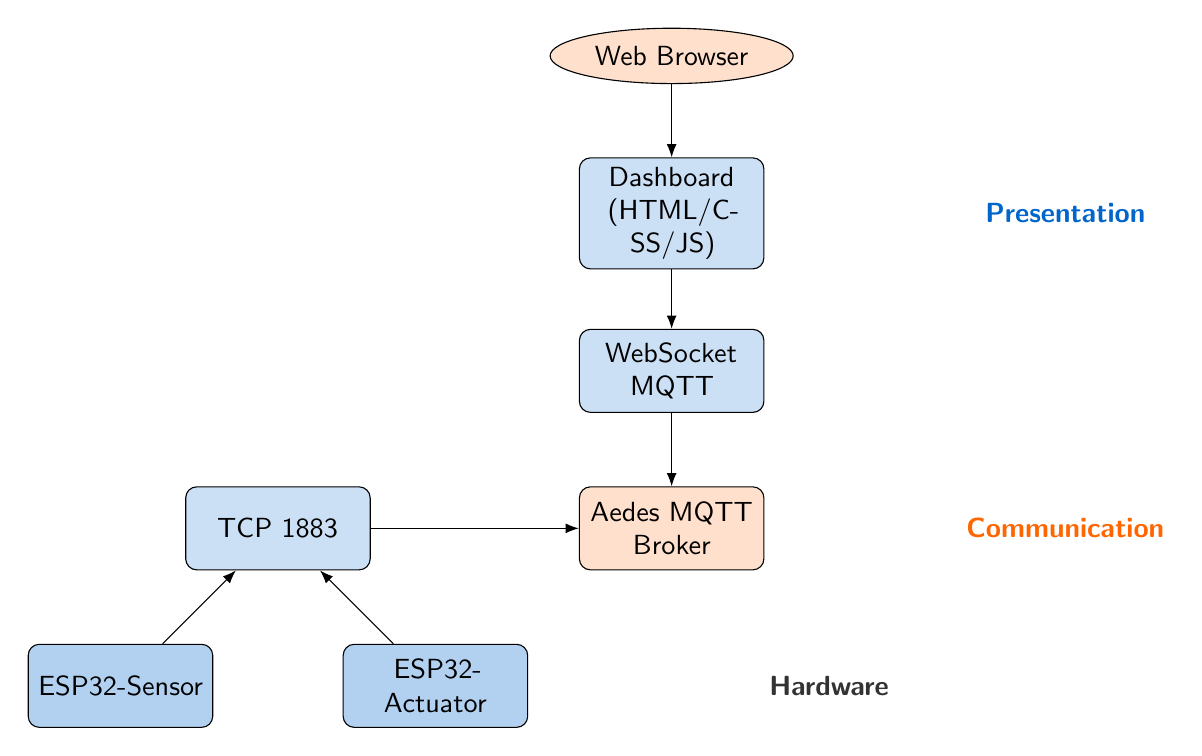
\begin{tikzpicture}[node distance=2cm, auto,
    block/.style={rectangle, draw, fill=primary!20, text width=6em, text centered, rounded corners, minimum height=3em},
    cloud/.style={draw, ellipse, shape=ellipse, fill=accent!20, minimum height=2em, text centered},
    line/.style={draw, -Latex}]
    
    % Presentation Layer
    \node [cloud] (browser) {Web Browser};
    \node [block, below of=browser] (dashboard) {Dashboard (HTML/CSS/JS)};
    \node [block, below of=dashboard] (websocket) {WebSocket MQTT};
    
    % Communication Layer
    \node [block, below of=websocket, fill=accent!20] (broker) {Aedes MQTT Broker};
    \node [block, left of=broker, xshift=-3cm] (tcp) {TCP 1883};
    
    % Hardware Layer
    \node [block, below of=tcp, xshift=-2cm, fill=primary!30] (sensor) {ESP32-Sensor};
    \node [block, below of=tcp, xshift=2cm, fill=primary!30] (actuator) {ESP32-Actuator};
    
    % Connections
    \path [line] (browser) -- (dashboard);
    \path [line] (dashboard) -- (websocket);
    \path [line] (websocket) -- (broker);
    \path [line] (tcp) -- (broker);
    \path [line] (sensor) -- (tcp);
    \path [line] (actuator) -- (tcp);
    
    % Layer labels
    \node [right of=dashboard, xshift=3cm, text=primary] {\textbf{Presentation}};
    \node [right of=broker, xshift=3cm, text=accent] {\textbf{Communication}};
    \node [right of=actuator, xshift=3cm, text=secondary] {\textbf{Hardware}};
\end{tikzpicture}
\caption{Three-Layer System Architecture}
\end{figure}

\subsection{Communication Flow}

The system implements bidirectional communication through the MQTT protocol:

\begin{itemize}
    \item \textbf{Sensor → Broker}: Publishes telemetry data every 5 seconds to \texttt{devices/\{id\}/telemetry}
    \item \textbf{Actuator ← Broker}: Subscribes to \texttt{device/\{id\}/gpio/set} for control commands
    \item \textbf{Dashboard $\leftrightarrow$ Broker}: WebSocket MQTT connection for real-time bidirectional communication
    \item \textbf{Gesture → GPIO}: MediaPipe hand gesture detection triggers automated GPIO control actions
\end{itemize}

\begin{figure}[h]
\centering
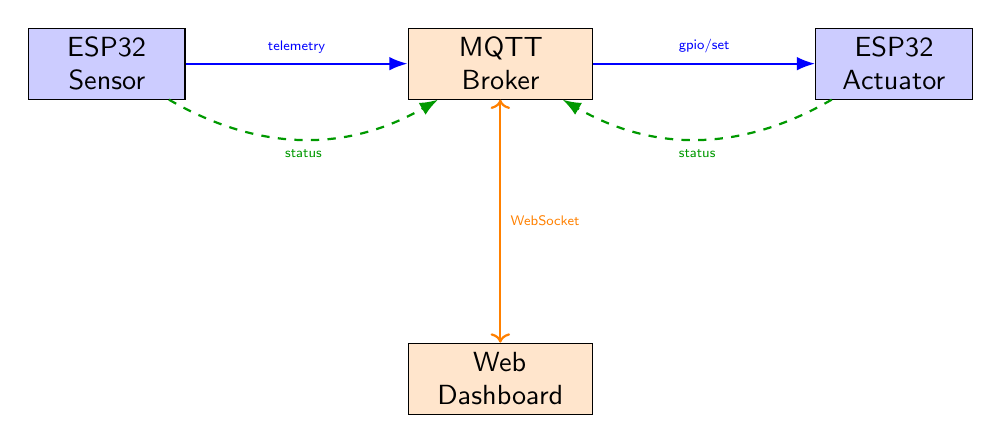
\begin{tikzpicture}[node distance=3cm, auto,
    device/.style={rectangle, draw, fill=blue!20, text width=5em, text centered, minimum height=2.5em},
    server/.style={rectangle, draw, fill=orange!20, text width=6em, text centered, minimum height=2.5em},
    arrow/.style={-Latex, thick}]
    
    \node [device] (sensor) {ESP32\\Sensor};
    \node [server, right of=sensor, xshift=2cm] (broker) {MQTT\\Broker};
    \node [device, right of=broker, xshift=2cm] (actuator) {ESP32\\Actuator};
    \node [server, below of=broker, yshift=-1cm] (dashboard) {Web\\Dashboard};
    
    % Arrows
    \draw [arrow, blue] (sensor) -- node[above] {\tiny telemetry} (broker);
    \draw [arrow, blue] (broker) -- node[above] {\tiny gpio/set} (actuator);
    \draw [arrow, orange, <->] (broker) -- node[right] {\tiny WebSocket} (dashboard);
    \draw [arrow, green!60!black, dashed] (sensor) to[bend right=30] node[below] {\tiny status} (broker);
    \draw [arrow, green!60!black, dashed] (actuator) to[bend left=30] node[below] {\tiny status} (broker);
\end{tikzpicture}
\caption{MQTT Message Flow Diagram}
\end{figure}

\subsection{Network Topology}

All devices connect to a central MQTT broker running on the Node.js server. The broker operates on two transport protocols:

\begin{itemize}
    \item \textbf{TCP}: Port 1883 for ESP32 device connections
    \item \textbf{WebSocket}: Port 3000/mqtt for browser-based dashboard access
\end{itemize}

\section{Hardware Components}

This section describes the hardware components used in this IoT system. The system consists of two types of ESP32-S3 based devices: a sensor device for environmental monitoring and an actuator device for remote control.

\begin{figure}[!htbp]
\centering
\includegraphics[width=0.6\textwidth]{hardware image/Yolo_Uno_ESP32-S3kit.png}
\caption{Yolo Uno ESP32-S3 Development Kit -- the main microcontroller board used for both sensor and actuator devices, featuring WiFi connectivity, multiple GPIO pins, and I2C support for sensor interfacing}
\end{figure}

\subsection{ESP32-Sensor Device}

The sensor device is responsible for environmental monitoring and real-time data publishing.

\subsubsection{Pin Connections}

\begin{lstlisting}[language=C, caption={DHT20 Sensor Connections}]
DHT20 Sensor:
  SDA  -> GPIO 11 (I2C Data Line)
  SCL  -> GPIO 12 (I2C Clock Line)
  VCC  -> 3.3V
  GND  -> GND

NeoPixel LED:
  DIN  -> GPIO 45 (Data Input)
  VCC  -> 5V
  GND  -> GND
\end{lstlisting}

\begin{figure}[!htbp]
\centering
\includegraphics[width=0.5\textwidth]{hardware image/DHT20Module.png}
\caption{DHT20 Temperature and Humidity Sensor Module -- an I2C-based digital sensor that measures both temperature and humidity with a single chip, connected via SDA (GPIO 11) and SCL (GPIO 12) lines}
\end{figure}

\subsubsection{Features}

The ESP32-Sensor integrates a DHT20 sensor that reads temperature and humidity measurements via the I²C bus every 5 seconds, providing continuous environmental monitoring. FreeRTOS task management organizes the firmware into separate concurrent tasks for sensor reading, MQTT communication, and UI updates, ensuring responsive operation. A WiFi configuration portal operating in Access Point mode with captive portal functionality enables easy initial setup without requiring code modifications.

Visual status indication through a NeoPixel LED displays connection status using intuitive color codes that communicate system state at a glance. Persistent configuration storage in NVS (Non-Volatile Storage) retains WiFi and MQTT credentials across power cycles, eliminating the need for reconfiguration. Built-in system diagnostics include an I²C scanner and health monitoring capabilities that facilitate troubleshooting and system verification.

\subsection{ESP32-Actuator Device}

The actuator device provides remote control capabilities for up to 8 independent GPIO channels.

\subsubsection{GPIO Pin Mapping}

\begin{lstlisting}[caption={GPIO Channel Assignments (from config.h)}]
GPIO 13 -> Channel 1 (Relay/LED)
GPIO 12 -> Channel 2 (Relay/LED)
GPIO 14 -> Channel 3 (Relay/LED)
GPIO 27 -> Channel 4 (Relay/LED)
GPIO 26 -> Channel 5 (Relay/LED)
GPIO 25 -> Channel 6 (Relay/LED)
GPIO 33 -> Channel 7 (Relay/LED)
GPIO 32 -> Channel 8 (Relay/LED)

NeoPixel LED:
  DIN  -> GPIO 45 (Status Indicator)
  VCC  -> 5V
  GND  -> GND
\end{lstlisting}

\begin{figure}[!htbp]
\centering
\includegraphics[width=0.6\textwidth]{hardware image/Relay.png}
\caption{8-Channel Relay Module -- allows the ESP32 actuator to control high-power devices such as lights, fans, and motors through isolated switching circuits}
\end{figure}

\begin{figure}[!htbp]
\centering
\includegraphics[width=0.5\textwidth]{hardware image/GPIO.png}
\caption{GPIO Testing Setup -- demonstrates LED indicators connected to GPIO output channels for visual verification of actuator commands before connecting to relays}
\end{figure}

\subsubsection{Features}

The ESP32-Actuator provides 8 independent GPIO channels capable of controlling relays, LEDs, motors, or any digital actuators, offering versatile output capabilities for diverse applications. MQTT command subscription enables real-time response to remote control commands with minimal latency. Heartbeat publishing sends periodic status messages every 20 seconds to maintain connection awareness and enable the dashboard to detect offline devices.

The web configuration interface utilizes the same WiFi Manager portal as the sensor device, ensuring consistent user experience across all system components. A NeoPixel connection status indicator visually communicates WiFi and MQTT connection state through color-coded feedback. Automatic reconnection logic provides robust error recovery for WiFi and MQTT disconnections, ensuring the system remains operational even in unstable network conditions.

\subsection{NeoPixel Status Codes}

Both devices use identical color-coding for connection status:

\begin{table}[h]
\centering
\begin{tabularx}{\textwidth}{lX}
\toprule
\textbf{Color} & \textbf{Status} \\
\midrule
Orange & Access Point mode active (waiting for configuration) \\
Red & Connecting to WiFi network \\
Blue & WiFi connected, MQTT broker connection in progress \\
Green & Fully operational (WiFi and MQTT connected) \\
\bottomrule
\end{tabularx}
\caption{NeoPixel LED Status Indicators}
\end{table}

\section{Firmware Architecture}

\subsection{FreeRTOS Task Structure}

The ESP32 firmware leverages FreeRTOS for concurrent task execution and resource management.

\subsubsection{ESP32-Sensor Tasks}

\begin{lstlisting}[language=C++, caption={Sensor Task Definitions}]
// Task 1: Sensor Reading (Priority: 2)
void TaskSensor(void *pvParameters) {
    while (1) {
        // Read DHT20 sensor via I2C
        float temp = dht.readTemperature();
        float humid = dht.readHumidity();
        
        // Update global state
        sensorState.temperature = temp;
        sensorState.humidity = humid;
        
        vTaskDelay(5000 / portTICK_PERIOD_MS);
    }
}

// Task 2: MQTT Communication (Priority: 3)
void TaskMQTT(void *pvParameters) {
    while (1) {
        // Maintain MQTT connection
        if (!mqtt.connected()) {
            reconnectMQTT();
        }
        mqtt.loop();
        
        // Publish telemetry
        publishTelemetry();
        
        vTaskDelay(1000 / portTICK_PERIOD_MS);
    }
}

// Task 3: UI Updates (Priority: 1)
void TaskUI(void *pvParameters) {
    while (1) {
        // Update NeoPixel based on connection state
        updateNeoPixelStatus();
        
        vTaskDelay(500 / portTICK_PERIOD_MS);
    }
}
\end{lstlisting}

\subsubsection{ESP32-Actuator Tasks}

\begin{lstlisting}[language=C++, caption={Actuator Task Definitions}]
// Task 1: MQTT Subscription (Priority: 3)
void TaskMQTT(void *pvParameters) {
    while (1) {
        if (!mqtt.connected()) {
            reconnectMQTT();
            // Subscribe to control topic
            mqtt.subscribe("device/+/gpio/set");
        }
        mqtt.loop();
        
        vTaskDelay(100 / portTICK_PERIOD_MS);
    }
}

// Task 2: Status Publishing (Priority: 2)
void TaskStatus(void *pvParameters) {
    while (1) {
        // Publish heartbeat every 20 seconds
        publishStatus();
        
        vTaskDelay(20000 / portTICK_PERIOD_MS);
    }
}

// Task 3: UI Updates (Priority: 1)
void TaskUI(void *pvParameters) {
    while (1) {
        updateNeoPixelStatus();
        
        vTaskDelay(500 / portTICK_PERIOD_MS);
    }
}
\end{lstlisting}

\subsection{Modular Code Organization}

The firmware follows a modular architecture with clear separation of concerns:

\begin{table}[h]
\centering
\begin{tabularx}{\textwidth}{lX}
\toprule
\textbf{Module} & \textbf{Responsibility} \\
\midrule
\texttt{config.h} & Hardware pin definitions and system constants \\
\texttt{types.h} & Data structures and type definitions \\
\texttt{globals.h} & Global variable declarations and object instances \\
\texttt{wifi\_manager.cpp} & WiFi connection management and AP mode \\
\texttt{mqtt\_handler.cpp} & MQTT client operations (publish/subscribe) \\
\texttt{neopixel\_handler.cpp} & WS2812B LED control and animations \\
\texttt{web\_server.cpp} & HTTP server for configuration interface \\
\texttt{config\_manager.cpp} & NVS flash storage for persistent settings \\
\texttt{tasks.cpp} & FreeRTOS task implementations (sensor only) \\
\texttt{diagnostics.cpp} & System health monitoring and I²C scanning (sensor only) \\
\bottomrule
\end{tabularx}
\caption{Firmware Module Organization}
\end{table}

\subsection{Configuration Management}

Both devices implement persistent configuration storage using ESP32's NVS (Non-Volatile Storage) system.

\begin{lstlisting}[language=C++, caption={Configuration Storage Structure}]
struct DeviceConfig {
    char wifiSSID[32];        // WiFi network name
    char wifiPassword[64];    // WiFi password
    char mqttServer[64];      // MQTT broker IP/hostname
    uint16_t mqttPort;        // MQTT broker port (default: 1883)
    char deviceName[32];      // Custom device name (optional)
    bool configured;          // Configuration complete flag
};

// Save configuration to NVS
bool saveConfig(DeviceConfig &config) {
    nvs_handle_t handle;
    nvs_open("config", NVS_READWRITE, &handle);
    
    nvs_set_str(handle, "wifiSSID", config.wifiSSID);
    nvs_set_str(handle, "wifiPass", config.wifiPassword);
    nvs_set_str(handle, "mqttServer", config.mqttServer);
    nvs_set_u16(handle, "mqttPort", config.mqttPort);
    nvs_set_str(handle, "deviceName", config.deviceName);
    nvs_set_u8(handle, "configured", config.configured ? 1 : 0);
    
    nvs_commit(handle);
    nvs_close(handle);
    
    return true;
}
\end{lstlisting}

\section{MQTT Communication Protocol}

\subsection{Topic Architecture}

The system implements a hierarchical MQTT topic structure for efficient message routing. Topics are organized by device ID with distinct patterns for sensor data (telemetry), device status, and control commands.

\begin{table}[h]
\centering
\begin{tabularx}{\textwidth}{llXl}
\toprule
\textbf{Topic Pattern} & \textbf{Direction} & \textbf{Purpose} & \textbf{QoS} \\
\midrule
\texttt{devices/\{id\}/telemetry} & ESP32→Server & Sensor readings and metrics & 0 \\
\texttt{devices/\{id\}/status} & ESP32→Server & Online/offline heartbeat & 1 \\
\texttt{device/\{id\}/gpio/set} & Server→ESP32 & GPIO control commands & 1 \\
\texttt{devices/\{id\}/cmd} & Server→ESP32 & Device commands (reboot, etc.) & 1 \\
\bottomrule
\end{tabularx}
\caption{MQTT Topic Structure (Actual Implementation)}
\end{table}

\textbf{Note on Topic Naming}: The system uses two slightly different prefixes for historical reasons—\texttt{devices/} (plural) for ESP32→Server topics and \texttt{device/} (singular) for Server→ESP32 control topics. This distinction helps identify message direction at a glance.

\subsection{Device ID Format}

Device IDs are automatically generated from the ESP32's unique MAC address:

Device identifiers are generated from the ESP32's unique MAC address:

\begin{itemize}
    \item \textbf{Sensor}: \texttt{ESP32-IOT-SENSOR-\{chipId\}}
    \item \textbf{Actuator}: \texttt{ESP32-IOT-ACTUATOR-\{chipId\}}
\end{itemize}

Where \texttt{\{chipId\}} is the last 4 hexadecimal digits of the MAC address (e.g., \texttt{a3f2}, \texttt{4e5c}).

\subsection{Message Formats}

\subsubsection{Sensor Telemetry}

\begin{lstlisting}[caption={Sensor Telemetry Message}]
{
  "tC": 24.5,          // Temperature in Celsius
  "tF": 76.1,          // Temperature in Fahrenheit
  "rh": 60.2,          // Relative Humidity (%)
  "timestamp": 1703012345678  // Unix timestamp (ms)
}
\end{lstlisting}

\subsubsection{Actuator Status}

\begin{lstlisting}[caption={Actuator Status Message}]
{
  "online": true,           // Connection status
  "ip": "192.168.1.150",   // Device IP address
  "rssi": -45,             // WiFi signal strength (dBm)
  "wifiMode": "STA",       // WiFi mode (STA/AP)
  "ts": 123456             // Timestamp
}
\end{lstlisting}

\subsubsection{GPIO Control Command}

\begin{lstlisting}[caption={GPIO Control Command}]
{
  "gpio": 5,    // GPIO channel number (1-8)
  "state": 1    // 0 = OFF, 1 = ON
}
\end{lstlisting}

\section{Web Dashboard}

\begin{figure}[!htbp]
\centering
\includegraphics[width=0.9\textwidth]{application-image/MainDashboard.png}
\caption{Main Dashboard Interface -- the primary control panel showing device status, live sensor readings, and navigation tabs for accessing different system functions}
\end{figure}

\subsection{Technology Stack}

The web dashboard is built with modern web technologies emphasizing simplicity and performance:

\begin{itemize}
    \item \textbf{Backend}: Node.js 16+, Express 4.x, Aedes MQTT Broker
    \item \textbf{Frontend}: Vanilla JavaScript (ES6+), CSS3, HTML5 (no frameworks)
    \item \textbf{AI/ML}: Google MediaPipe Hands library
    \item \textbf{Communication}: WebSocket-MQTT for real-time updates
\end{itemize}

\subsection{Modular JavaScript Architecture}

The frontend is organized into 6 independent modules:

\begin{table}[h]
\centering
\begin{tabularx}{\textwidth}{llX}
\toprule
\textbf{Module} & \textbf{Lines} & \textbf{Responsibility} \\
\midrule
\texttt{automation.js} & 288 & Rule-based automation engine \\
\texttt{devices.js} & 365 & Device management and GPIO control \\
\texttt{gestures.js} & 388 & MediaPipe integration and gesture detection \\
\texttt{mqtt.js} & 193 & WebSocket MQTT client and message handling \\
\texttt{ui.js} & 156 & UI initialization and tab management \\
\texttt{events.js} & 91 & Event logging system with export functionality \\
\bottomrule
\end{tabularx}
\caption{Frontend Module Organization}
\end{table}

\subsection{Dashboard Features}

\subsubsection{0. Main Dashboard Overview}

The main dashboard provides a unified view of the entire IoT fleet at a glance.

\begin{figure}[!htbp]
\centering
\includegraphics[width=0.9\textwidth]{application-image/MainDashboard.png}
\caption{Main Dashboard -- displays system statistics (total devices, online count, sensor/automation counts) at the top, followed by device preview cards showing real-time telemetry and quick GPIO controls for up to 2 devices}
\end{figure}

Key dashboard sections:

\begin{itemize}
    \item \textbf{Statistics Cards}: Four metric cards show total devices, online devices, active sensors, and configured automation rules with large numbers and icons
    \item \textbf{Device Preview}: Displays first 2 online devices with condensed information cards
    \item \textbf{Quick Controls}: Each device card includes 3 quick-access GPIO toggle switches
    \item \textbf{Navigation}: Six tab buttons (Dashboard, Device Fleet, Gesture Control, Automation, Events, MQTT Docs) enable rapid access to specialized interfaces
    \item \textbf{Status Indicator}: Header shows MQTT broker connection status with real-time device count
\end{itemize}

The dashboard updates automatically every second, refreshing device telemetry, online status, and GPIO states without requiring manual page reload.

\subsubsection{1. Devices Tab}

The Devices Tab provides real-time monitoring of all connected devices through visual cards displaying each device's status. Live telemetry delivers auto-updating temperature and humidity readings that refresh every 2 seconds. Color-coded online/offline indicators use green badges for connected devices and red badges for offline status, providing immediate system health visibility. Device information includes the device ID, type classification (sensor/actuator), IP address, and WiFi signal strength in dBm, enabling network diagnostics and device identification.

\begin{figure}[!htbp]
\centering
\includegraphics[width=0.9\textwidth]{application-image/DeviceManagement.png}
\caption{Device Management Tab -- displays all connected ESP32 devices as cards showing their online/offline status, device type (sensor or actuator), IP address, and WiFi signal strength}
\end{figure}

\subsubsection{2. Control Tab}

The remote GPIO control interface provides individual ON/OFF toggle switches for each of the 8 GPIO channels, enabling precise control over connected actuators. Modern toggle switches provide clear visual feedback with green illumination for ON state and gray for OFF state. WebSocket-based MQTT communication enables sub-100ms response times from click to actuator response. A device selection dropdown facilitates control in multi-actuator environments where multiple ESP32-Actuator devices operate simultaneously.

\subsubsection{3. Gestures Tab}

AI-powered gesture recognition leverages MediaPipe Hands to detect 21 hand landmarks, enabling sophisticated hand tracking capabilities. 

\begin{figure}[!htbp]
\centering
\includegraphics[width=0.9\textwidth]{application-image/AI-Webcam.png}
\caption{AI Gesture Control Interface -- shows live webcam feed with MediaPipe hand tracking overlay, detected gesture display, and confidence percentage. The interface includes Start Camera button and gesture rule configuration panel}
\end{figure}

The gesture system supports five distinct patterns:

\begin{itemize}
    \item \textbf{Fist}: All fingers closed -- useful for "grip" or "stop" actions
    \item \textbf{Palm}: All fingers extended -- ideal for "open" or "activate" commands
    \item \textbf{Point Up}: Index finger extended -- precise directional control
    \item \textbf{Victory}: Index and middle fingers extended -- dual-state toggling
    \item \textbf{Thumbs Up}: Thumb pointing upward -- confirmation or approval actions
\end{itemize}

Each gesture maps to GPIO actions through configurable rules. The interface displays live camera feed with hand skeleton overlay, current detected gesture with confidence percentage, and rule management panel for creating gesture-to-action mappings.

\subsubsection{4. Automation Tab}

The automation engine enables conditional device control based on sensor thresholds without manual intervention.

\begin{figure}[!htbp]
\centering
\includegraphics[width=0.9\textwidth]{application-image/Automation.png}
\caption{Automation Rules Interface -- allows creation of IF-THEN rules such as "IF temperature > 30°C THEN turn ON fan (GPIO 1)". Shows rule list with enable/disable toggles and edit/delete controls}
\end{figure}

Rule structure follows IF-THEN logic:

\begin{itemize}
    \item \textbf{Condition (IF)}: Source device + parameter (temperature/humidity/RSSI) + operator (>, <, >=, <=, ==) + threshold value
    \item \textbf{Action (THEN)}: Target device + GPIO pin (1-8) + state (ON/OFF)
    \item \textbf{Auto-Toggle}: Optional automatic reversal when condition no longer met
\end{itemize}

Example rules: "IF temperature > 30°C THEN GPIO 1 ON" activates cooling when hot. "IF humidity < 40\% THEN GPIO 2 ON" starts humidifier when dry. The automation engine evaluates rules every 2 seconds, executing actions only on state transitions to prevent repeated triggering.

\subsubsection{5. Events Tab}

Comprehensive activity logging records all system events with timestamps, severity levels, and detailed messages.

\begin{figure}[!htbp]
\centering
\includegraphics[width=0.9\textwidth]{application-image/Events Log.png}
\caption{Events Log Tab -- chronological list of system events including device connections, MQTT messages, GPIO commands, and automation triggers. Supports export to JSON for external analysis}
\end{figure}

Event categories include:

\begin{itemize}
    \item \textbf{INFO}: Device connections, WiFi status, routine operations
    \item \textbf{SUCCESS}: Successful command execution, rule triggers
    \item \textbf{WARNING}: Connection degradation, missed heartbeats
    \item \textbf{ERROR}: Communication failures, invalid messages
\end{itemize}

The log maintains up to 1000 recent events in memory with circular buffer management. Export functionality generates JSON file containing full event history with ISO 8601 timestamps for archival and analysis purposes.

Live preview functionality overlays real-time hand landmark detection on the camera feed, providing immediate visual feedback during gesture recognition.

\subsubsection{4. Automation Tab}

The conditional rule engine executes actions automatically when sensor data meets specified thresholds, enabling autonomous system operation. Supported comparison operators include greater than, less than, equal to, not equal to, greater than or equal to, and less than or equal to, providing flexible condition evaluation. Auto-toggle functionality optionally sends an automatic OFF command after a specified delay, useful for temporary activations.

Practical examples demonstrate the system's capabilities: when temperature exceeds 30°C, GPIO 1 activates a cooling fan; when humidity drops below 40\%, GPIO 2 engages a humidifier; when temperature falls below 18°C, GPIO 3 powers a heater. These automation rules eliminate the need for constant manual monitoring while maintaining optimal environmental conditions.

\begin{figure}[!htbp]
\centering
\includegraphics[width=0.9\textwidth]{application-image/Automation.png}
\caption{Automation Rules Tab -- allows users to create conditional rules that trigger GPIO actions based on sensor thresholds, such as turning on a fan when temperature exceeds a set value}
\end{figure}

\subsubsection{5. Events Tab}

Comprehensive system logging captures all MQTT messages, device connections, GPIO actions, gestures, and automation triggers in a unified event stream. Precise timestamps with millisecond accuracy enable detailed analysis of system behavior and timing relationships between events. Color-coded event types provide visual distinction, making it easy to identify different categories of system activity at a glance.

Export functionality allows downloading the complete event log as a JSON file for offline analysis, archival, or integration with external tools. Real-time updates ensure events appear instantly as they occur, providing immediate visibility into system operations and facilitating rapid debugging when issues arise.

\begin{figure}[!htbp]
\centering
\includegraphics[width=0.9\textwidth]{application-image/Events Log.png}
\caption{Events Log Tab -- records all system activities including MQTT messages, device connections, GPIO state changes, gesture detections, and automation triggers with timestamps}
\end{figure}

\subsection{Responsive Design}

The dashboard implements a mobile-first responsive design using CSS Grid layout for flexible device card arrangement that adapts to different screen sizes. Breakpoints optimize the interface for desktop, tablet, and mobile screens, ensuring usability across all form factors. A dark theme reduces eye strain during extended monitoring sessions while maintaining excellent readability and contrast. Touch-friendly design features large buttons and interactive elements sized appropriately for touch interfaces, making the system accessible on smartphones and tablets without requiring precise cursor control.

\subsection{Documentation Tab}

The dashboard includes a built-in documentation tab that provides system integration guides and reference information directly within the interface.

\begin{figure}[!htbp]
\centering
\includegraphics[width=0.9\textwidth]{application-image/DocumentationTab.png}
\caption{Documentation Tab -- provides built-in help, API reference, and integration guides directly within the dashboard}
\end{figure}

\subsection{Dashboard Performance and Usability}

The web dashboard achieves real-time responsiveness through several optimization techniques:

\textbf{Efficient Updates}: JavaScript modules use requestAnimationFrame for smooth visual updates and minimize DOM manipulation by batching changes. WebSocket connection maintains persistent bidirectional channel with the MQTT broker, eliminating HTTP polling overhead.

\textbf{Modular Architecture}: Six independent JavaScript modules (\texttt{events.js}, \texttt{mqtt.js}, \texttt{devices.js}, \texttt{gestures.js}, \texttt{automation.js}, \texttt{ui.js}) load asynchronously and communicate through well-defined interfaces. This separation of concerns simplifies debugging and enables independent module testing.

\textbf{Responsive Design}: CSS Grid and Flexbox layouts adapt seamlessly to screen sizes from 320px (mobile) to 4K displays. Media queries optimize card arrangements and typography at breakpoints: mobile (<768px), tablet (768-1100px), desktop (>1100px).

\textbf{Accessibility Features}: Gesture control provides alternative input method for users with limited mobility. High-contrast dark theme meets WCAG 2.1 AA standards. Touch targets exceed 44x44px minimum for reliable interaction on mobile devices.

\section{Web Dashboard Screenshots}

\subsection{ESP32-Sensor Main Dashboard}

\begin{figure}[!htbp]
\centering
\includegraphics[width=0.9\textwidth]{application-image/Esp32-Sensors-MainDashboard.jpg}
\caption{ESP32-Sensor Main Dashboard View -- displays real-time temperature (26.87°C) and humidity (61.32\% RH) readings with device status indicators showing online connection, WiFi signal strength, and system uptime}
\end{figure}

The sensor dashboard presents environmental data in an intuitive card-based layout. Temperature displays in both Celsius and Fahrenheit with trend indicators. Humidity percentage includes comfort zone visualization. Device status section shows connection quality (WiFi RSSI: -47 dBm indicates excellent signal), heap memory usage, and continuous uptime tracking.

\subsection{ESP32-Sensor Telemetry Monitoring}

\begin{figure}[!htbp]
\centering
\includegraphics[width=0.9\textwidth]{application-image/Esp32-Sensors-Sensors Monitor Tab.jpg}
\caption{Sensor Monitor Tab -- detailed telemetry view showing all sensor readings, quality metrics, and system diagnostics in a comprehensive monitoring interface}
\end{figure}

The telemetry tab provides expanded view of all sensor metrics including data quality score (calculated from sensor response time and value validation), free heap memory monitoring for memory leak detection, and WiFi signal strength tracking for connectivity diagnostics.

\subsection{ESP32-Actuator Main Dashboard}

\begin{figure}[!htbp]
\centering
\includegraphics[width=0.9\textwidth]{application-image/Esp32-Actuator-MainDashboard.jpg}
\caption{ESP32-Actuator Main Dashboard -- shows online actuator device with 8 GPIO control channels, each with individual ON/OFF toggle switches for remote control}
\end{figure}

The actuator dashboard emphasizes control functionality with prominent toggle switches for each GPIO channel. Visual feedback through color-coded switches (green=ON, gray=OFF) provides immediate state confirmation. Device information panel displays connection status, IP address, and system health metrics.

\subsection{ESP32-Actuator GPIO Control Interface}

\begin{figure}[!htbp]
\centering
\includegraphics[width=0.9\textwidth]{application-image/Esp32-Actuator-GPIO Control Tab.jpg}
\caption{GPIO Control Tab -- dedicated interface for managing all 8 GPIO channels with large toggle switches optimized for both mouse and touch interaction}
\end{figure}

The full GPIO control tab presents all eight channels in an organized grid layout. Each channel includes GPIO number label, current state indicator, and toggle control. The interface updates in real-time as commands are sent via MQTT, providing immediate visual confirmation of relay states.

\subsection{MQTT Broker Integration}

\begin{figure}[!htbp]
\centering
\includegraphics[width=0.45\textwidth]{application-image/Esp32-Sensors-MQTT Broker Tab.jpg}
\hfill
\includegraphics[width=0.45\textwidth]{application-image/Esp32-Actuator-MQTT Broker Tab.jpg}
\caption{MQTT Broker Configuration Screens -- both sensor (left) and actuator (right) devices use identical captive portal interfaces for easy broker setup}
\end{figure}

The MQTT broker configuration interface provides:

\begin{itemize}
    \item \textbf{Broker Discovery}: Automatic mDNS scanning detects local MQTT brokers on the network
    \item \textbf{Manual Entry}: IP address and port fields allow custom broker configuration
    \item \textbf{Connection Testing}: Built-in test validates broker connectivity before saving
    \item \textbf{Security Options}: Optional pairing token field for device authentication
    \item \textbf{Status Feedback}: Real-time connection status with colored indicators
\end{itemize}

\section{Node.js Server Implementation}

\subsection{Server Architecture}

The Node.js server serves three primary roles:

\begin{enumerate}
    \item \textbf{MQTT Broker}: Aedes-based message broker for device communication
    \item \textbf{HTTP Server}: Express application serving static dashboard files
    \item \textbf{Device Registry}: Automatic discovery and tracking of ESP32 devices
\end{enumerate}

\subsection{Dual-Protocol MQTT}

The server exposes MQTT over two transport protocols:

\begin{table}[h]
\centering
\begin{tabularx}{\textwidth}{lXl}
\toprule
\textbf{Protocol} & \textbf{Purpose} & \textbf{Port} \\
\midrule
TCP & Native MQTT for ESP32 devices & 1883 \\
WebSocket & Browser-based dashboard connection & 3000/mqtt \\
\bottomrule
\end{tabularx}
\caption{MQTT Transport Protocols}
\end{table}

\subsection{Server Code Structure}

\begin{lstlisting}[caption={Node.js Server Implementation}]
const express = require('express');
const aedes = require('aedes')();
const net = require('net');
const ws = require('websocket-stream');
const http = require('http');

// Create HTTP server
const app = express();
const server = http.createServer(app);

// Serve static dashboard files
app.use(express.static('public'));
app.use(express.json());

// TCP MQTT broker (port 1883)
const mqttServer = net.createServer(aedes.handle);
mqttServer.listen(1883, () => {
    console.log('[MQTT] TCP broker:      mqtt://localhost:1883');
});

// WebSocket MQTT (port 3000/mqtt)
ws.createServer({ server: server, path: '/mqtt' }, aedes.handle);

// Device registry
const devices = new Map();

// MQTT message handler
aedes.on('publish', (packet, client) => {
    const topic = packet.topic;
    const payload = packet.payload.toString();
    
    // Update device registry
    if (topic.includes('/status')) {
        const deviceId = topic.split('/')[1];
        devices.set(deviceId, {
            lastSeen: Date.now(),
            online: true
        });
    }
});

// Start HTTP server
server.listen(3000, () => {
    console.log('[HTTP] Dashboard:       http://localhost:3000');
    console.log('[MQTT] WebSocket:       ws://localhost:3000/mqtt');
});
\end{lstlisting}

\subsection{Device Auto-Discovery}

The server automatically tracks devices based on MQTT activity:

\begin{itemize}
    \item \textbf{First Message}: Device added to registry upon first publish
    \item \textbf{Heartbeat Monitoring}: Devices marked offline if no message received in 30 seconds
    \item \textbf{Reconnection}: Devices automatically restored to online status when reconnecting
    \item \textbf{Registry Persistence}: In-memory Map structure (can be extended to database)
\end{itemize}

\section{MediaPipe Gesture Recognition}

\begin{figure}[!htbp]
\centering
\includegraphics[width=0.9\textwidth]{application-image/AI-Webcam.png}
\caption{Gesture Recognition Interface -- shows the webcam feed with MediaPipe hand landmark overlay detecting finger positions in real-time for touchless device control}
\end{figure}

\subsection{Implementation Details}

The gesture recognition system leverages Google's MediaPipe Hands library:

\begin{lstlisting}[caption={MediaPipe Initialization}]
const hands = new Hands({
    locateFile: (file) => {
        return `https://cdn.jsdelivr.net/npm/@mediapipe/hands/${file}`;
    }
});

hands.setOptions({
    maxNumHands: 1,           // Track single hand
    modelComplexity: 1,       // Balance speed/accuracy
    minDetectionConfidence: 0.7,
    minTrackingConfidence: 0.7
});

hands.onResults((results) => {
    if (results.multiHandLandmarks) {
        const landmarks = results.multiHandLandmarks[0];
        const gesture = detectGestureFromLandmarks(landmarks);
        
        if (gesture) {
            executeGestureAction(gesture);
        }
    }
});
\end{lstlisting}

\subsection{Gesture Detection Algorithm}

Each gesture is detected through geometric analysis of hand landmarks:

\begin{lstlisting}[caption={Gesture Detection Logic}]
function detectGestureFromLandmarks(landmarks) {
    // Calculate finger extension states
    const fingers = {
        thumb: isThumbExtended(landmarks),
        index: isFingerExtended(landmarks, 8),
        middle: isFingerExtended(landmarks, 12),
        ring: isFingerExtended(landmarks, 16),
        pinky: isFingerExtended(landmarks, 20)
    };
    
    // Fist: All fingers closed
    if (!fingers.thumb && !fingers.index && 
        !fingers.middle && !fingers.ring && !fingers.pinky) {
        return 'fist';
    }
    
    // Palm: All fingers extended
    if (fingers.thumb && fingers.index && 
        fingers.middle && fingers.ring && fingers.pinky) {
        return 'palm';
    }
    
    // Peace: Index and middle extended
    if (!fingers.thumb && fingers.index && 
        fingers.middle && !fingers.ring && !fingers.pinky) {
        return 'peace';
    }
    
    // Thumbs Up/Down: Thumb position analysis
    if (fingers.thumb && !fingers.index && 
        !fingers.middle && !fingers.ring && !fingers.pinky) {
        return isThumbUp(landmarks) ? 'thumbs_up' : 'thumbs_down';
    }
    
    return null;
}
\end{lstlisting}

\subsection{Configuration Options}

The MediaPipe initialization in the code uses these settings:

\begin{itemize}
    \item \textbf{maxNumHands}: 1 (tracks single hand for reliability)
    \item \textbf{modelComplexity}: 1 (balanced speed and accuracy)
    \item \textbf{minDetectionConfidence}: 0.7 (70\% confidence threshold)
    \item \textbf{minTrackingConfidence}: 0.7 (70\% tracking threshold)
    \item \textbf{Landmark Points}: 21 hand keypoints tracked per hand
\end{itemize}

\section{System Configuration}

\subsection{Timing Configuration}

These timing values are defined in the firmware configuration files:

\begin{table}[h]
\centering
\begin{tabularx}{\textwidth}{lXl}
\toprule
\textbf{Parameter} & \textbf{Description} & \textbf{Value} \\
\midrule
Sensor Read Interval & DHT20 reading frequency & 5000 ms \\
UI Update Interval & NeoPixel LED refresh rate & 500 ms \\
MQTT Loop Interval & MQTT client processing rate & 100 ms \\
Button Long Press & Duration for config reset & 3000 ms \\
\bottomrule
\end{tabularx}
\caption{Firmware Timing Configuration (from config.h)}
\end{table}

\section{Setup and Deployment}

\subsection{Prerequisites}

\begin{itemize}
    \item \textbf{Hardware}: ESP32-S3 development boards, DHT20 sensor, WS2812B LEDs
    \item \textbf{Software}: 
    \begin{itemize}
        \item PlatformIO Core 6.0+ or VS Code with PlatformIO extension
        \item Node.js 16.0.0 or higher
        \item npm 8.x or higher
    \end{itemize}
    \item \textbf{Network}: WiFi router (all devices on same network)
    \item \textbf{Development}: Git for version control
\end{itemize}

\subsection{Installation Steps}

\subsubsection{Step 1: Setup Web Server}

\begin{lstlisting}[language=bash, caption={Server Installation}]
# Navigate to server directory
cd Web-Server/server

# Install Node.js dependencies
npm install

# Start the server
npm start

# Expected output:
# ============================================================
# ESP32 IoT Fleet Management System - Server v2.0
# ============================================================
# [HTTP] Dashboard:       http://localhost:3000
# [MQTT] TCP broker:      mqtt://localhost:1883
# [MQTT] WebSocket:       ws://localhost:3000/mqtt
# ============================================================
\end{lstlisting}

\begin{warningbox}[Important]
Note your computer's IP address on the local network (e.g., \texttt{192.168.1.100}). This will be needed for ESP32 MQTT configuration. Do not use \texttt{localhost} or \texttt{127.0.0.1} as ESP32 devices cannot resolve these.
\end{warningbox}

\subsubsection{Step 2: Flash ESP32-Sensor Firmware}

\begin{lstlisting}[language=bash, caption={Sensor Firmware Upload}]
# Navigate to sensor project
cd ESP32-Sensor

# Build firmware
pio run

# Upload to ESP32 (connect via USB)
pio run --target upload

# Open serial monitor for debugging
pio device monitor
\end{lstlisting}

\subsubsection{Step 3: Configure ESP32-Sensor}

\begin{enumerate}
    \item Connect to WiFi AP: \texttt{ESP32-IOT-SENSOR-xxxx} (password: \texttt{12345678})
    \item Open web browser: \texttt{http://192.168.4.1}
    \item Enter configuration:
    \begin{itemize}
        \item WiFi SSID: Your home WiFi network name
        \item WiFi Password: Your WiFi password
        \item MQTT Server: Your computer's IP (e.g., \texttt{192.168.1.100})
        \item MQTT Port: \texttt{1883}
        \item Device Name: Optional custom name
    \end{itemize}
    \item Click "Save Configuration"
    \item Device will reboot and connect automatically
\end{enumerate}

\subsubsection{Step 4: Flash ESP32-Actuator Firmware}

\begin{lstlisting}[language=bash, caption={Actuator Firmware Upload}]
# Navigate to actuator project
cd ESP32-Actuator

# Build and upload firmware
pio run --target upload

# Monitor serial output
pio device monitor
\end{lstlisting}

\subsubsection{Step 5: Configure ESP32-Actuator}

Follow the same configuration process as the sensor device using WiFi AP \texttt{ESP32-IOT-ACTUATOR-xxxx}.

\subsubsection{Step 6: Access Dashboard}

\begin{enumerate}
    \item Open web browser
    \item Navigate to: \texttt{http://localhost:3000}
    \item Devices should appear in the device grid within 30 seconds
    \item Green "Online" badge indicates successful connection
\end{enumerate}

\section{Troubleshooting Guide}

\subsection{Devices Show Offline}

\textbf{Symptoms}: Devices appear in dashboard but show red "Offline" badge.

\textbf{Solutions}:
\begin{itemize}
    \item Verify MQTT server IP in ESP32 configuration (must be computer's LAN IP, not \texttt{localhost})
    \item Wait 30 seconds for initial connection
    \item Check NeoPixel LED shows green (fully connected)
    \item Verify Windows Firewall allows Node.js on port 1883
    \item Test MQTT connection with command-line tools:
\end{itemize}

\begin{lstlisting}[language=bash, caption={MQTT Testing}]
# Install mosquitto client
npm install -g mqtt

# Subscribe to all device topics
mosquitto_sub -h localhost -t "devices/#" -v
\end{lstlisting}

\subsection{GPIO Control Not Working}

\textbf{Symptoms}: Clicking GPIO buttons produces no response.

\textbf{Solutions}:
\begin{itemize}
    \item Ensure actuator device shows "Online" status
    \item Check browser console for JavaScript errors (F12)
    \item Verify MQTT WebSocket connection is established
    \item Refresh browser page to reset connection
    \item Confirm topic subscription in serial monitor: \texttt{device/\{id\}/gpio/set}
\end{itemize}

\subsection{Sensor Not Publishing Data}

\textbf{Symptoms}: No temperature/humidity data appears in dashboard.

\textbf{Solutions}:
\begin{itemize}
    \item Verify DHT20 wiring (SDA=GPIO11, SCL=GPIO12, 3.3V, GND)
    \item Access diagnostics endpoint: \texttt{http://192.168.4.1/api/diagnostics}
    \item Check I²C address (DHT20 should be 0x38)
    \item Monitor serial output for sensor reading errors
    \item Test with different DHT20 sensor to rule out hardware failure
\end{itemize}

\subsection{Gesture Recognition Issues}

\textbf{Symptoms}: Camera shows video but no gestures detected.

\textbf{Solutions}:
\begin{itemize}
    \item Grant camera permissions when browser prompts
    \item Use \texttt{http://localhost:3000} (not IP address) for HTTPS requirement
    \item Improve lighting conditions for better landmark detection
    \item Use Google Chrome or Microsoft Edge (best MediaPipe compatibility)
    \item Hold hand 30-60 cm from camera
    \item Ensure single hand is visible (multi-hand detection may confuse system)
\end{itemize}

\section{Future Enhancements}

\subsection{Planned Features}

\begin{itemize}
    \item \textbf{Database Integration}: PostgreSQL or MongoDB for long-term telemetry storage and historical analysis
    \item \textbf{User Authentication}: Multi-user support with role-based access control
    \item \textbf{Cloud MQTT}: Integration with AWS IoT Core or Azure IoT Hub for remote access
    \item \textbf{Mobile Application}: React Native companion app for iOS and Android
    \item \textbf{Voice Control}: Amazon Alexa and Google Assistant integration
    \item \textbf{Advanced Sensors}: Support for energy monitoring (current/voltage sensors)
    \item \textbf{OTA Updates}: Over-the-air firmware updates for ESP32 devices
    \item \textbf{Data Visualization}: Grafana dashboards for advanced analytics
    \item \textbf{Security}: TLS/SSL encryption for MQTT with certificate-based authentication
    \item \textbf{Internationalization}: Multi-language support for global deployment
\end{itemize}

\subsection{Scalability Improvements}

\begin{itemize}
    \item Load balancing for high-volume deployments
    \item Clustering support for MQTT broker redundancy
    \item Time-series database optimization for IoT workloads
    \item Edge computing capabilities for local decision-making
\end{itemize}

\section{Educational Value}

This project provides comprehensive learning opportunities across multiple domains:

\subsection{Embedded Systems}

\begin{itemize}
    \item FreeRTOS multi-tasking and synchronization
    \item I²C peripheral communication
    \item GPIO digital output control
    \item Non-volatile storage (NVS) management
    \item Interrupt handling and hardware timers
    \item Memory management on constrained devices
\end{itemize}

\subsection{IoT Protocols}

\begin{itemize}
    \item MQTT publish/subscribe architecture
    \item WebSocket bidirectional communication
    \item HTTP RESTful API design
    \item JSON data serialization
    \item Quality of Service (QoS) levels
\end{itemize}

\subsection{Web Development}

\begin{itemize}
    \item Modern vanilla JavaScript (ES6+)
    \item Modular CSS architecture
    \item Responsive web design principles
    \item Real-time data visualization
    \item DOM manipulation and event handling
\end{itemize}

\subsection{Artificial Intelligence}

\begin{itemize}
    \item Computer vision with MediaPipe
    \item Hand landmark detection and tracking
    \item Gesture classification algorithms
    \item Real-time ML inference in browser
\end{itemize}

\subsection{Software Engineering}

\begin{itemize}
    \item Modular code organization
    \item Separation of concerns
    \item Version control with Git
    \item Build systems (PlatformIO, npm)
    \item Documentation best practices
\end{itemize}

\section{Conclusion}

The ESP32 IoT Fleet Management System represents a complete, production-ready IoT ecosystem that successfully integrates hardware, firmware, middleware, and software components into a cohesive platform. The system demonstrates technical excellence through robust FreeRTOS implementation, efficient MQTT communication, and modern web technologies that work seamlessly together. Innovation is evident in the AI-powered gesture control using MediaPipe, enabling hands-free operation that enhances accessibility and user experience.

Usability improvements include web-based configuration that eliminates hardcoded credentials and simplifies deployment across different network environments. The modular architecture supports unlimited devices with minimal overhead, proving the system's scalability for real-world applications. Reliability is ensured through automatic reconnection mechanisms, persistent configuration storage, and comprehensive error handling that maintains operation even under adverse conditions.

The project successfully achieves its goals of creating an educational yet practical platform for understanding full-stack IoT development. From low-level embedded programming with FreeRTOS to high-level web application design with modern JavaScript, the system encompasses the complete technology stack. With over 3000 lines of carefully architected code across firmware and software components, this platform provides a solid foundation for further enhancement and deployment in production environments including home automation, industrial monitoring, and smart building management.

\appendix

\section{Source Code Repository}

Complete source code, documentation, and hardware schematics are available at:

\begin{center}
\url{https://github.com/leonathn/FinalProject_ESP32S3_LocalMQTT-NodeJs-FreeRTOS}
\end{center}

\section{Pinout Diagrams}

\subsection{ESP32-S3 Pinout Reference}

Refer to official Espressif documentation for complete pinout:
\url{https://docs.espressif.com/projects/esp-idf/en/latest/esp32s3/hw-reference/esp32s3/user-guide-devkitc-1.html}

\subsection{DHT20 Sensor Pinout}

\begin{table}[h]
\centering
\begin{tabular}{ll}
\toprule
\textbf{Pin} & \textbf{Function} \\
\midrule
1 & SDA (I²C Data) \\
2 & GND \\
3 & VCC (3.3V) \\
4 & SCL (I²C Clock) \\
\bottomrule
\end{tabular}
\caption{DHT20 Sensor Pin Configuration}
\end{table}

\section{License Information}

This project is licensed under the MIT License:

\begin{lstlisting}[basicstyle=\ttfamily\footnotesize]
MIT License

Copyright (c) 2025 Final Project - Embedded Systems

Permission is hereby granted, free of charge, to any person obtaining
a copy of this software and associated documentation files (the
"Software"), to deal in the Software without restriction, including
without limitation the rights to use, copy, modify, merge, publish,
distribute, sublicense, and/or sell copies of the Software, and to
permit persons to whom the Software is furnished to do so, subject to
the following conditions:

The above copyright notice and this permission notice shall be
included in all copies or substantial portions of the Software.

THE SOFTWARE IS PROVIDED "AS IS", WITHOUT WARRANTY OF ANY KIND,
EXPRESS OR IMPLIED, INCLUDING BUT NOT LIMITED TO THE WARRANTIES OF
MERCHANTABILITY, FITNESS FOR A PARTICULAR PURPOSE AND NONINFRINGEMENT.
IN NO EVENT SHALL THE AUTHORS OR COPYRIGHT HOLDERS BE LIABLE FOR ANY
CLAIM, DAMAGES OR OTHER LIABILITY, WHETHER IN AN ACTION OF CONTRACT,
TORT OR OTHERWISE, ARISING FROM, OUT OF OR IN CONNECTION WITH THE
SOFTWARE OR THE USE OR OTHER DEALINGS IN THE SOFTWARE.
\end{lstlisting}

\section{References}

\begin{thebibliography}{99}

\bibitem{esp32s3}
Espressif Systems.
\textit{ESP32-S3 Technical Reference Manual}.
Version 1.5, 2023.
\url{https://www.espressif.com/sites/default/files/documentation/esp32-s3_technical_reference_manual_en.pdf}

\bibitem{freertos}
Real Time Engineers Ltd.
\textit{FreeRTOS Reference Manual}.
Version 10.4.0, 2021.
\url{https://www.freertos.org/Documentation/RTOS_book.html}

\bibitem{mqtt}
OASIS.
\textit{MQTT Version 5.0 Specification}.
2019.
\url{https://docs.oasis-open.org/mqtt/mqtt/v5.0/mqtt-v5.0.html}

\bibitem{mediapipe}
Google LLC.
\textit{MediaPipe Hands Solution}.
2023.
\url{https://google.github.io/mediapipe/solutions/hands.html}

\bibitem{aedes}
Moscajs Project.
\textit{Aedes MQTT Broker Documentation}.
Version 0.51.0, 2023.
\url{https://github.com/moscajs/aedes}

\bibitem{platformio}
PlatformIO Labs.
\textit{PlatformIO Documentation}.
2023.
\url{https://docs.platformio.org/}

\bibitem{dht20}
Aosong Electronics.
\textit{DHT20 Digital Temperature and Humidity Sensor Datasheet}.
Version 1.0, 2020.

\bibitem{ws2812b}
Worldsemi.
\textit{WS2812B Intelligent Control LED Datasheet}.
Version 2.0, 2018.

\end{thebibliography}

\end{document}
